\chapter{SYSTEM DESIGN}
\label{igen}
Human are very intelligent in understanding natural language text and finding the information using reasoning. In our case, this information is IOCs from security reports, articles, and malware reports. However, it is very hard for the machines to do the information extraction with high accuracy and coverage. 

iGen identifies sentences likely containing IOCs using a set of regular expressions. Then, IOCs are efficiently captured with high accuracy using CNN-based model.  iGen tries to automatically identify the patterns or features which are frequent in IOC and non-IOC sentences. Architectural design of the iGen is shown in Figure~\ref{fig:architecture}.


\begin{figure*}[tb]
\centering
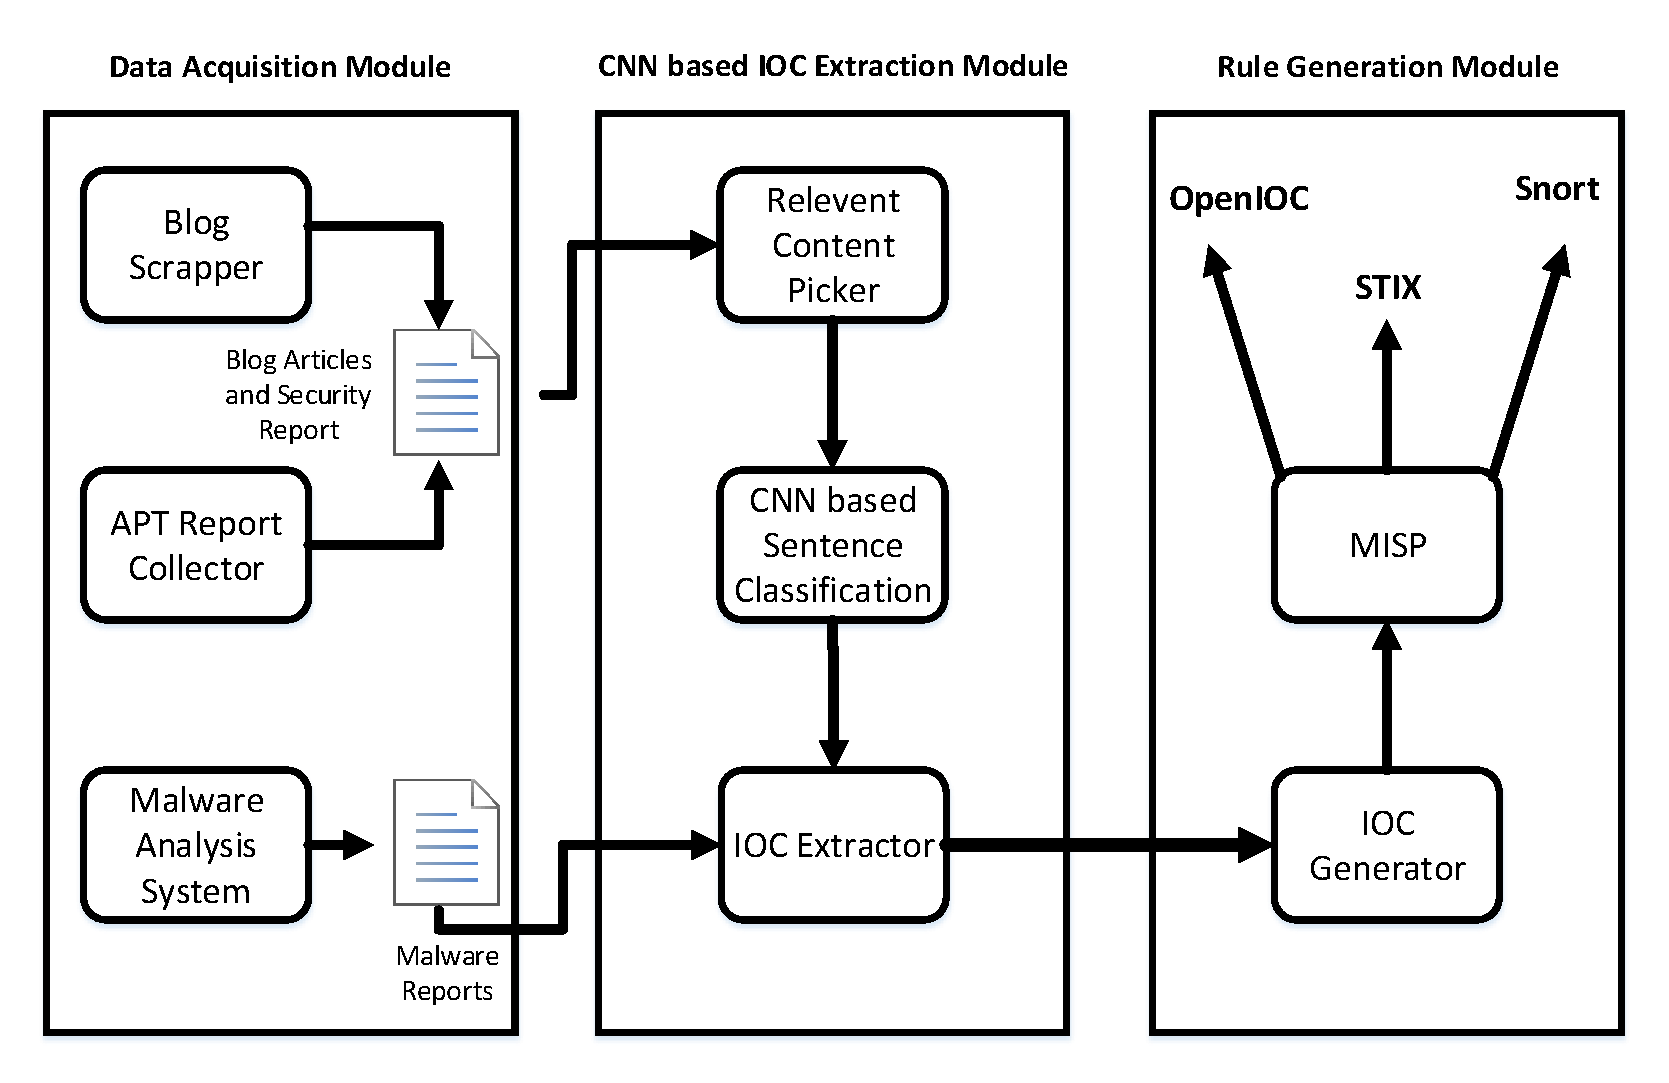
\includegraphics [width=\linewidth]{Architecture.pdf}
\caption{iGen Architecture Overview.}
\label{fig:architecture}
\end{figure*}


\subsection{Architecture Overview}
iGen consists of 3 modules from left to right: 1) data acquisition module, 2) CNN based IOC extraction module, and 3) rule generation module. Data acquisition module consists of three sub-module: Blog Scrapper (BS), APT Report Collector (ARC), and Cuckoo Malware Analysis System (CMAS). BS is a collection of crawlers based on the HTML structure of the different blogs. For instance, there is a dedicated crawler which is continuously looking for new articles on Symantec public blog~\cite{symantecblog}. Similarly, ARC continuously looks for new whitepapers and reports about APT campaigns at ``APTNotes''~\cite{apt} database. CMAS collects malware reports from Cuckoo~\cite{bayer}, which is an open source malware analysis system. 

 Then, these reports are passed to an IOC extraction module based on the type of the report. Because blog articles and security reports are written in English and follow natural language semantics, these are given as input to the Relevant Content Picker (RCP) component for further processing. RCP parses those reports, cleans the text, and selects the sentences having likely IOCs using regular expressions. Then, these sentences are fed to the CNN based Sentence Classification (CSC) module for classification into two classes: IOC and non-IOC sentences.  Whereas, malware reports follow JSON format with no natural language semantics involved. This makes it easier for IOC Extractor (IE) to extract IOCs based on the structure of the JSON report. Simultaneously, IE also performs regular expressions based extraction of IOCs from the sentences that are classified by CNN based Sentence Classifier (CSC) as IOC sentences.    

Next step is to organize IOCs extracted from each report into one event (malware or APT campaign) is done by IOC Generator (IG). For example, “Monkeys.exe” and “200.125.133.28” are the IOCs related to the event CozyDuke APT campaign~\cite{cozyduke}. Then, these events are stored and managed by Malware Information Sharing Platform (MISP)~\cite{misp}. MISP also provide an additional functionality to iGen by converting these event into different output formats like STIX, OpenIOC, Snort etc. 
    
\subsection{Data Collection}
There are two sources of TI data: internal, e.g., malware analysis reports or network traces, or external, such as technical blogs or security reports. Examples of external sources include the Kaspersky whitepapers~\cite{kaspersky}, Symantec blog~\cite{symantecblog} etc. Recently, thousands of threats are reported every day, which has been broadly reported by the security companies in the form of APT/security reports~\cite{daly} or blog articles and aggressively collected by different organizations. For the scope of our research, we collected 1000 security reports and 1500 blog articles from different security organizations. All these reports and articles are published from year 2011 to 2017. Our scrapper collected information from more than 20 prominent security organization like Verizon, Symantec etc.

To bootstrap our research, we also collected around 35,000 malware reports from our in-house Cuckoo Malware Analysis System (CMAS)~\cite{oktavianto}. MAS provided some detailed results outlining what malware did when executed inside an isolated environment. While substantial volume of security reports, blog articles and malware reports are collected and analyzed, however it only constitutes a small part of the bigger IOC landscape. Summary of our dataset is in Table 1.  

\begin{table}[tb]
\caption{Summary of Dataset} % title of Table
\centering % used for centering table
\begin{tabular}{c c c} % centered columns (4 columns)
\hline\hline %inserts double horizontal lines
Dataset Type & Dataset Source & Number of articles/ reports \\ [0.5ex] % inserts table
%heading
\hline % inserts single horizontal line
Security Reports & External & 1000 \\ % inserting body of the table
Technical Blog Articles & External & 1500 \\
Malware Analysis Reports & Internal & 35000 \\[1ex] % [1ex] adds vertical space
\hline %inserts single line
\end{tabular}
\label{table:dataset} % is used to refer this table in the text
\end{table}

\section{Data Acquisition Module}
This module collects information from different sources. Because of the scalable nature of the module, new data sources can be added as well. This module scrap related web pages, APT report from different sites. Simultaneously, it continuously collects malware reports from our internal CMAS as well. All the sub-modules of data acquisition module are described in the following.

\subsection{Blog Scrapper (BS)}
iGen blog scraper is designed to continuously monitor a list of security blogs and collect their articles. BS first scraps all its current articles before it is set to monitoring mode to identify new ones for each blog site. Most of the blog articles on most of the blog sites have a particular page id associated with it. BS keep track of the range of page ids that are already scrapped by it. In monitor mode, it looks for new articles. If there are no new articles posted on the blog sites, then BS changes its mode to idle and want back to monitor mode after $n$ days. For our research, we have set the $n$ as 7 days. BS also collects the reports if there is any PDF report link within the blog article.



\subsection{APT Report Collector (ARC)}
APT report collector consists of autonomous data crawler, which continuously check for new reports and whitepapers at APTNotes database. It also keeps track of the already scrapped reports to avoid duplication. Around 1000 APT campaign report are collected till date.

\subsection{Cuckoo Malware Analysis System (CMAS)}
For our research, we have a Cuckoo malware analysis system (CMAS)~\cite{bayer} for automating analysis of suspicious files. CMAS monitors the behaviour of the malicious processes while running in an isolated environment. In other words, if we submit any suspicious file to it and in a matter of seconds CMAS will provide us back some detailed results outlining what such file did when executed inside an isolated environment. Features of CMAS are : 
\begin{itemize}
 \item[$\bullet$ ] Analyze different type of malicious files (executables, document expoits, malicious websites etc.).
  \item[$\bullet$ ] Dump and analyze network traffic, even when encrypted.
  \item[$\bullet$ ] Trace API calls and general behavior of the file.
\end{itemize}

For scope of this research, around 35000 malware were submitted and analyzed by CMAS. Later, these reports were further used for IOCs extraction.

\section{IOC Extraction Module}
After the collection of dataset, the next step is to clean the data, select relevant content, and find IOCs with high degree of confidence. In this module, Relevant Content Picker (RCP) cleans the data by removing the terms with no semantic meaning such as stop words, etc. RCP also finds sentences which are likely to contain IOCs. Afterwards, CNN based Sentence Classification (CSC) and IOC Extractor (IE) identify the IOC sentences and extract the IOCs from them respectively. 



\subsection{Relevant Content Picker (RCP)}
Relevant Content Picker extracts text from PDF and HTML documents. In our implementation, the RCP uses the python library ``pdfminer''~\cite{pdfminer} to extract the text from the PDF reports and ``beautifulsoup''~\cite{beautifulsoup} to obtain content from HTML pages as well to find links to security reports in blog articles. RCP scans for URLs with an extension ``.pdf'' in the blog articles to identify security reports linked with the blog articles. If RCP finds any PDF report linked with blog article, it sends it to PDFminer for further processing. After the collection of content, the next step is to remove the terms or token with no semantic meaning such as stop words. Stop words extremely common words which would appear to be of little value in terms of semantic significance like ``a'', ``an'', ``the'' etc. Removing stopwords is a part of the data cleaning process. Third and final step is to look for sentences which are likely to have IOCs. This part is done by finding the sentences which have patterns like IP, hostname, URL, filename, registry, email, filepath etc. These are patterns are identified using the set of regular expressions. Some sample regular expressions are shown in Table~\ref{table:reg}. 




\begin{figure*}[tb]
\centering
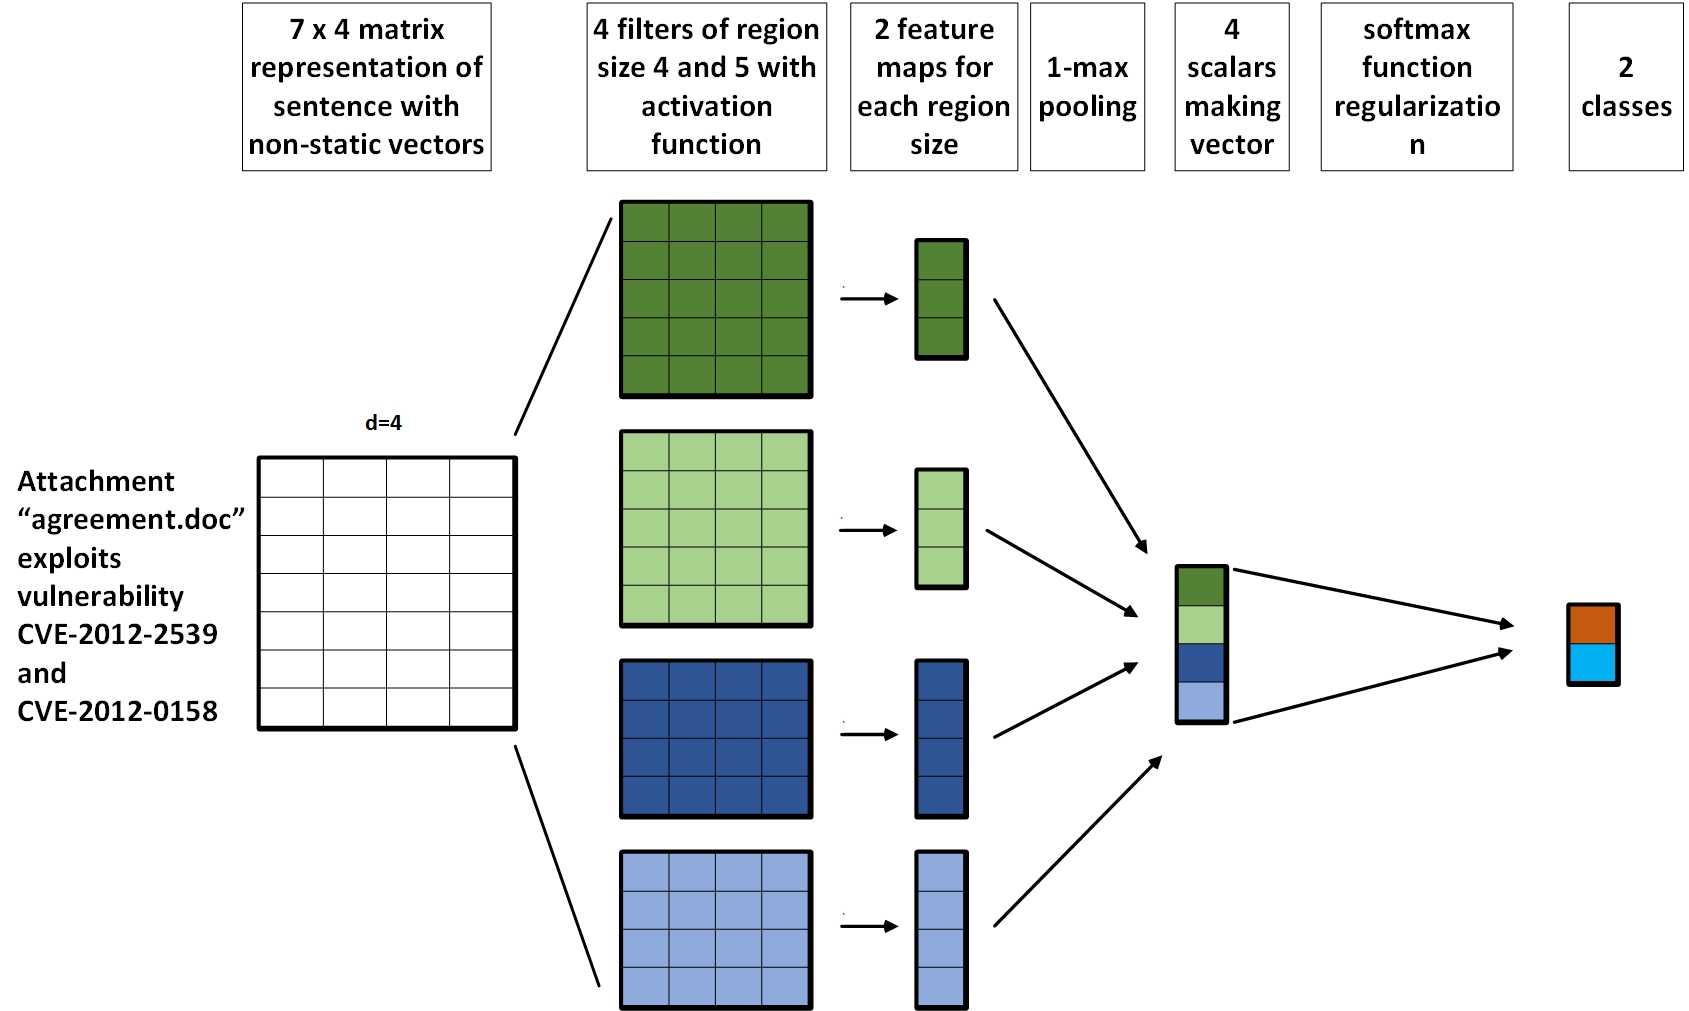
\includegraphics [width=\linewidth]{CNN_sentence.jpg}
\caption{Architecture of CNN based sentence classification model. We show two filter region sizes: 4 and 5, each of which has 2 filters. Filters or kernels accomplish convolutions and apply activation functions on the sentence matrix and generate (variable-length) feature maps; 1-max pooling is performed over each map, i.e., the largest number from each feature map is recorded. Thus a univariate feature vector is generated from all 4 maps, and these 4 features are concatenated to form a feature vector for the penultimate layer. The final softmax layer then receives this feature vector as input and uses it to classify the sentence; here we are performing binary classification and hence depict two possible output states.}
\label{fig:CNNsentence}
\end{figure*}

\subsection{CNN based Sentence Classification (CSC)}




The model architecture of CNN based Sentence Classification (CSC), shown in figure~\ref{fig:CNNsentence}, is a minor variant of the CNN architecture suggested by Kim ~\cite{kim}. First step of CSC involves converting all the words in the sentences into their respective word vector or embedding.
Let $\mathbf{S}_i \in \mathbb{R}^{d}$ be the  word vector of dimensionality $d$ corresponding to the $i$-th word or token in the sentence. A sentence of length $l$ is characterized as
\begin{equation}
\mathbf{S}_{1:l} = \mathbf{S}_1 \oplus \mathbf{S}_2 \oplus \ldots \oplus \mathbf{S}_l,
\end{equation}
where concatenation operator is defined as $\oplus$. 




The first step is to calculate word embedding of $S_i$ based on our dataset. We call this layer as embedding layer, which maps vocabulary word indices into low-dimensional vector representations. $X$ is our embedding matrix that we learn during training. We initialize it using a random uniform distribution~\cite{claessen}. $tf.nn.embedding\_lookup$~\cite{tensorflowapi} function in tensorflow creates the actual embedding operation. The result of the embedding operation is a 3-dimensional tensor of shape $[None, sequencelength, embeddingsize]$.
TensorFlow's convolutional conv2d~\cite{tensorflowapi} operation expects a 4-dimensional tensor with dimensions corresponding to batch, width, height, and channel. The results of our embedding does not contain the channel dimension, so we add it manually, leaving us with a layer of shape $[None, sequencelength, embeddingsize, 1]$.

A word embedding $\mathbf{X} \colon words \rightarrow \mathbf{R}^n$  is a paramaterized function mapping words in some language to high-dimensional vectors (perhaps 200 to 500 dimensions). For example 
\begin{equation}
\mathbf{X}(``malware") = (0.2,-0.4,0.7,\ldots)
\end{equation}

Characteristically, the function is a lookup table, parameterized by a matrix, $\theta$, with a row for each word: $\mathbf{X}_\theta(w_n)= \mathbf{X}_n = \theta_n$.

$\mathbf{X}$ is initialized to have random vectors for each word. It learns to have meaningful vectors in order to classify the sentences into IOC and non-IOC sentences.

Let $\mathbf{S}_{i:j}$ refer to a sentence of length $j-i+1$ or the concatenation of words vectors $\mathbf{S}_i = \mathbf{X}_\theta(w_i), \mathbf{S}_{i+1} = \mathbf{X}_\theta(w_{i+1}), \ldots, \mathbf{S}_{j}=\mathbf{X}_\theta(w_j)$.
Single convolution consist of a \emph{filter} $\mathbf{w} \in \mathbb{R}^{h\times d}$, which is applied to a window of $h$ words to automatically generate a new feature. For example, a feature $f_i$ is generated from a window of words $\mathbf{S}_{i:i+h-1}$ by
\begin{equation}
f_i = f(\mathbf{w} \cdot \mathbf{S}_{i:i+h-1} + c).
\end{equation}
Here bais term $c \in \mathbb{R}$ is added and $f$ is a non-linear function such as the rectified linear unit (ReLU) or hyperbolic tangent (tanh). Filter is applied to each possible window of words in the sentence $\{\mathbf{S}_{1:h}, \mathbf{S}_{2:h+1}, \ldots, \mathbf{S}_{l-h+1:l}\}$ to produce a \emph{feature map}
\begin{equation}
\mathbf{f} = [f_1, f_2, \ldots, f_{l-h+1}],
\end{equation}
where $\mathbf{f} \in \mathbb{R}^{l-h+1}$. We then apply a 1-max pooling operation~\cite{ranzato} over the feature map and take the maximum value $\dot{f} = \max \{\mathbf{f}\}$ as the feature corresponding to this particular filter. Intuition behind this is to capture the most important feature---one with the highest value---for each feature map. This kind of approach works naturally with variable sentence lengths. 

Above described process extracts $one$ feature from $one$ filter. The model uses multiple filters with different region size to obtain multiple features. These features creates the penultimate layer and the final layer is a fully connected softmax layer whose output is the probability distribution over labels (in our case, “IOC sentence” or “non-IOC sentence”).

In our model, we have fine-tuned word vectors via backpropagation~\cite{rumelhart}. For regularization~\cite{zou} we used dropout~\cite{srivastava} on the penultimate layer with a constraint on $l_2$-norms~\cite{ng} of the weight vectors~\cite{hinton}. Dropout helps in co-adaptation of hidden units by randomly dropping out---i.e., setting to zero---a proportion $p$ of the hidden units during foward-backpropagation. That is, given the penultimate layer $\mathbf{y} = [\dot{f}_1, \ldots, \dot{f}_n]$ where $n$ is total number of filters). Instead of using
\begin{equation}
z = \mathbf{w} \cdot \mathbf{y} + b
\end{equation}
during forward propagation for output unit $y$, dropout uses
\begin{equation}
z = \mathbf{w} \cdot (\mathbf{y}\circ\mathbf{r}) + b,
\end{equation}
where $\circ$ is the element-wise multiplication operator and $\mathbf{r} \in \mathbb{R}^n$ is a `masking' vector of Bernoulli random variables with probability $p$ of being 1. During the training, gradients\cite{friedman} are backpropagated only through the unmasked units. During the testing, all learned weight vectors are scaled by $p$ such that $\dot{\mathbf{w}} = p\mathbf{w}$, and $\dot{\mathbf{w}}$ is used  to score new sentences without dropout.

\begin{table}[tb]
\caption{Sample Regular Expressions used by Relevant Content Picker (RCP) and IOC Extractor (IE).} % title of Table
\centering % used for centering table
\begin{tabular}{c c} % centered columns (4 columns)
\hline\hline %inserts double horizontal lines
Type of Regular Expression & Regular Expression \\ [0.5ex] % inserts table
%heading
\hline % inserts single horizontal line
Email & \verb/\b([a-z][_a-z0-9-.]+@[a-z0-9-]+\.[a-z]+)\b/ \\ % inserting body of the table
IP & \verb/\b(\d{1,3}\.\d{1,3}\.\d{1,3}\.\d{1,3})\b/ \\
MD5  & \verb/\b([a-f0-9]{32}|[A-F0-9]{32})\b/ \\ % [1ex] adds vertical space
CVE  & \verb/\b(CVE\-[0-9]{4}\-[0-9]{4,6})\b/ \\[1ex]
\hline %inserts single line
\end{tabular}
\label{table:reg} % is used to refer this table in the text
\end{table}


\subsection{IOC Extractor (IE)}
As shown in Figure~\ref{fig:architecture}, IOC extractor takes malware report as well the sentences which are classified as IOC sentences by CSC sub-system as input. Since, malware reports doesn$'$t have any natural language semantics, we skipped running RCP and CSC sub-systems on them. Additionally, MAS is run only on the malware files that implies all the indicator/tokens (e.g., file hashes, emails, etc.) are malicious.

In case of malware reports, structure of JSON file is used to extract the IOCs. Whereas, regex as shown in Table~\ref{table:reg} were used to extract the IOC from the sentences. These are different type of IOCs collected by the IE: URL, host, IP, email, MD5, SHA1, SHA256, CVE, registry, filename, and filepath. Next step is to bundle the IOCs related to one event/malware together.



\section{Rule Generation System}
This system works on the managing the related IOCs and convert them into different output formats so that these IOCs based formats can be directly deployed on the security infrastructure. Currently, iGen supports STIX, OpenIOC, snort, suricata, and BRO formats. Rule generation system has two sub-systems: IOC Generator (IG) and Malware Information Sharing Platform (MISP)~\cite{misp}.

\subsection{IOC Generator (IG)}
IOC generator takes IOCs from IE and bind them together into one IOC event if they are coming from the same report. This sub-system creates event into MISP acceptable JSON format. Then, this JSON is submitted to MISP. 

\subsection{Malware Information Sharing Platform (MISP)}
MISP is an open source software for sharing, storing and correlating IOCs of targeted attacks. MISP benefits security community by showing collaborative knowledge about existing malware or threats. The aim of this trusted platform is to help improving the counter-measures used against targeted attacks and set-up preventive actions and detection. It stores data in a structured format and allows automated use of the database to feed detection systems or forensic tools. For example, it generates rules from IOCs (e.g. IP addresses, domain names, hashes of malicious files, filenames, filepath etc.) for different Network Intrusion Detection Systems (NIDS) like snort, suricata etc. MISP adds an extra feature of generating diverse rules from the IOCs collected from different data sources.

